\section{Trade-off between Quality of Processing and Resource Cost}
\label{sec:cost}
When the user is willing to accept approximate results, it is possible to use the \sic metric to expose
a trade-off between the quality of processing and resource cost. 
If we maintain a stable amount of processing resources, increasing the number of deployed queries
leads to a reduction of the resource cost per query. 
When the percentage of cost reduction is greater than the reduction in processing quality (\ie SIC
values) there is a cost advantage by adding more queries. 

The difference in cost, $\Delta(cost)$, is calculated as:
\begin{align}
	\Delta(cost) = \frac{C_{base}-C_x}{C_{base}}
\end{align}
where $C_{base}$ is the base resource cost for the initial deployment and $C_x$ is the resource cost of
deploying $x$ queries.

The difference in quality of processing, $\Delta(QoP)$, is calculated as:
\begin{align}
	\Delta(QoP) = \frac{QoP_{base}-QoP_x}{QoP_{base}}
\end{align}

where $QoP_{base}$ is the quality of processing value for the starting deployment and $QoP_x$ is the
quality of processing achieved after deploying $x$ queries.

The deployment of new queries is considered to be advantageous when:
\begin{align}
	\Delta(QoP)>\Delta(Cost)
\end{align}
\begin{figure} 
\centering 
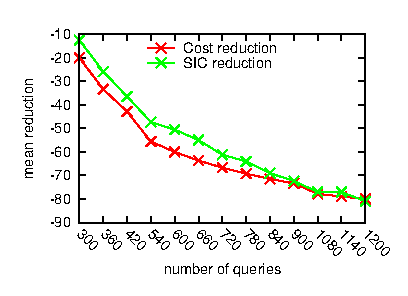
\includegraphics[width=0.6\textwidth]{img/tesi/cost2}  
\caption{Trade-off between the reduction of resource cost per query and the reduction in quality of
processing, as expressed by mean SIC values.}
\label{fig:tradeoff-mean}
\end{figure}
The difference between the reduction in cost and quality of processing is inversely proportional to the
number of queries. The more queries are added, the lower the cost advantage, until a point is reached,
at which increasing the number of queries is no longer beneficial.
% A user can keep adding new queries until this point is reached, until the difference goes under a certain
% threshold, or until a minimum SIC values is reached.
A user may add more queries until this point is reached or the difference is below a given threshold or
minimal \sic value.

\subsection*{Experimental Results}

For the trade-off evaluation, the data from Figure~\ref{fig:scalability:queries} is used. The cost of the
infrastructure remains fixed so the resource cost per query can be calculated as the inverse of the
number of queries: $1/N_{queries}$.

Figure~\ref{fig:tradeoff-mean} shows the mean \sic value as the quality of processing metric. The base
case has 180 queries and, at each step, 60 more queries are deployed. The graph shows how, with 300
queries, there is almost an 8\% difference between the reduction in quality of processing and the
resource cost reduction.
This difference grows smaller as more queries are deployed until a ``tipping point'' is reached with
approximately 900 queries. From this point onwards, adding more queries does not result in further
benefit.
% Figure~\ref{fig:tradeoff-q95} shows the same trend but uses the Q.95-Q.05 metric as the
% quality-of-service indicator.

%%\mnote{what else?}


% \begin{figure}[h!]
% \centering
% 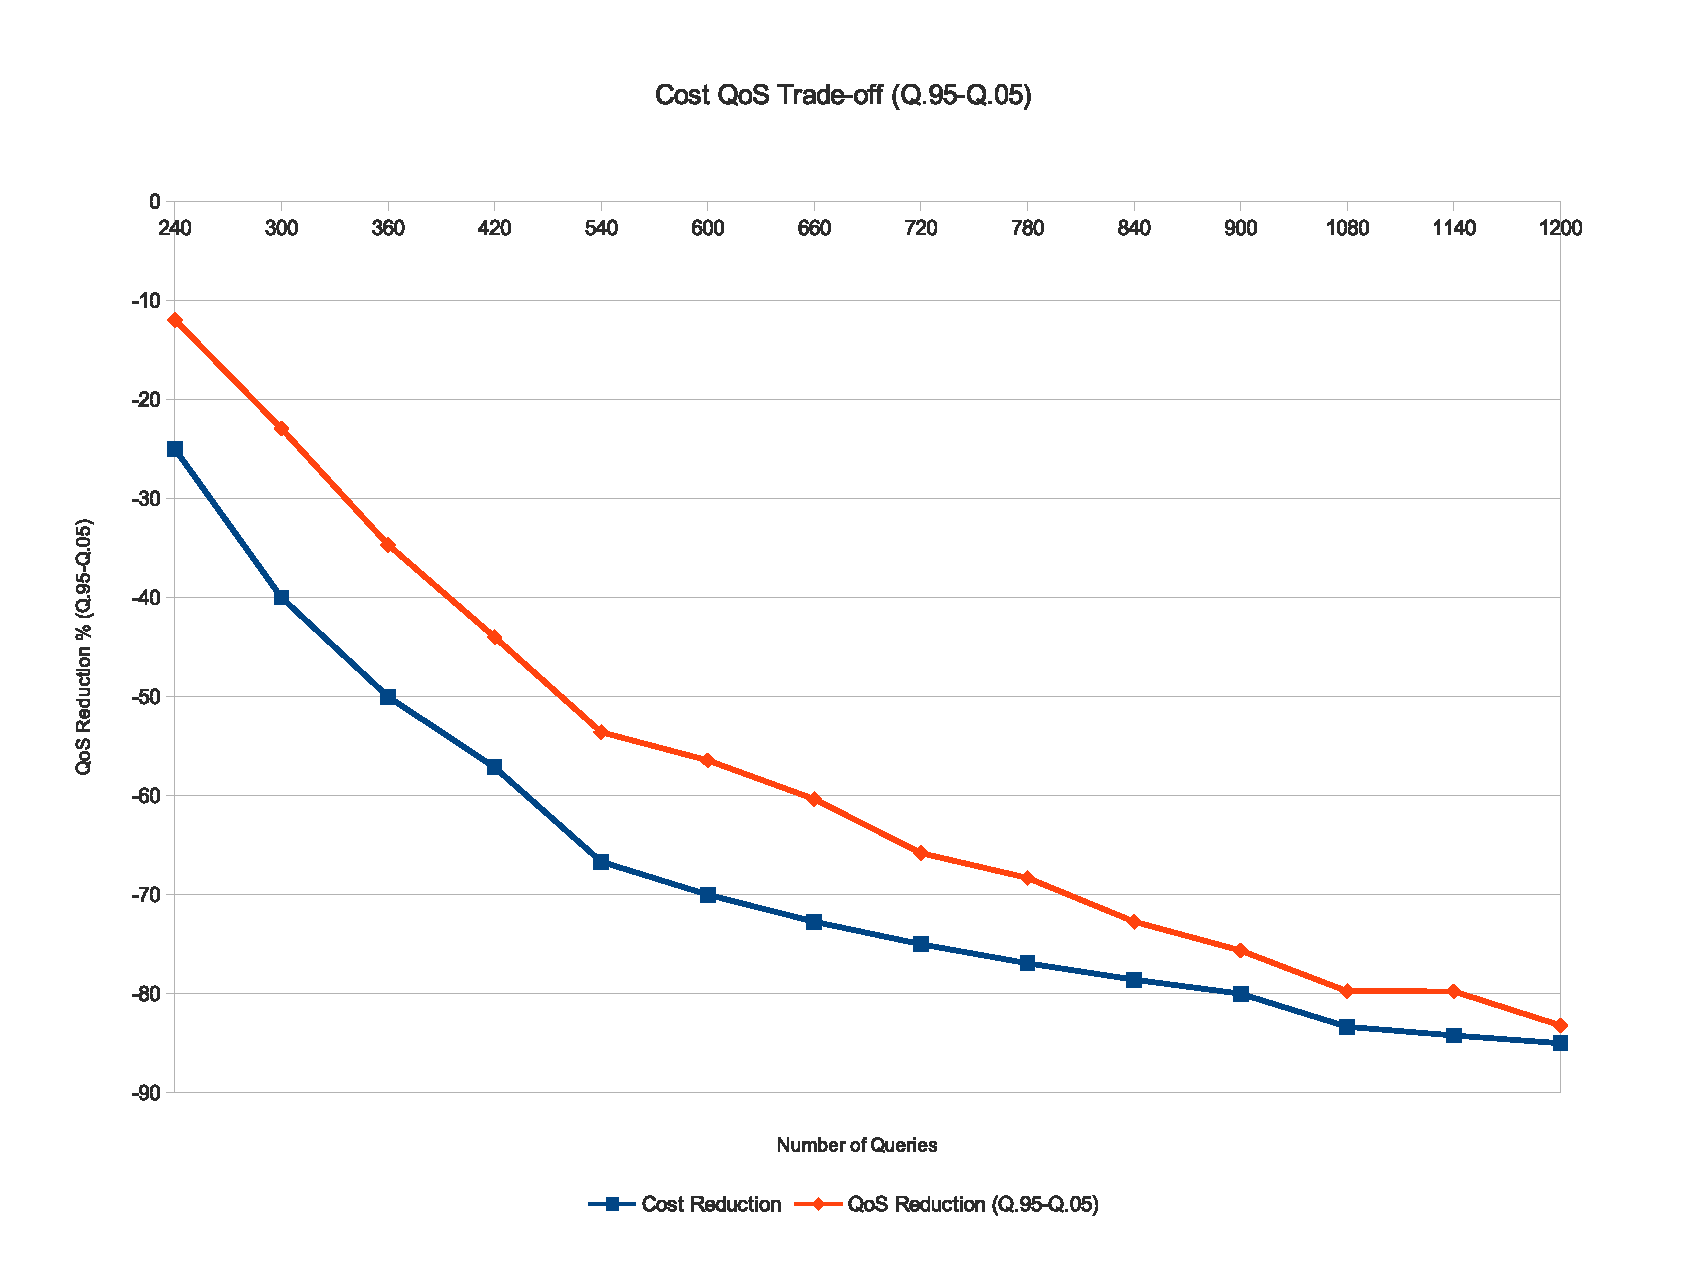
\includegraphics[width=0.6\textwidth]{img/tesi/tradeoff-q95} 
% \caption{Trade-off between the reduction of cost per query and redution in Qos expressed as Q.95-Q.05 SIC
% values.}
% \label{fig:tradeoff-q95}
% \end{figure}

%\clearpage
 